\section{Diagnostic limits on a production model and a shallow instance}
\label{sec:diagnostics}

\subsection{Production model}
\label{sec:production}

\paragraph{Setup.}
BlockViT-v2 is a spectral--spatial segmentation model from a companion
tokenization study (anonymous, under review): a linear per-pixel reduction
$942\to K=64$ ($\Cf=61{,}108$ parameters) followed by a 12-layer ViT of
embedding width $M$ with a convolutional decoder
($\Cg=18{,}271{,}540$ at $M=192$; $\Cg/\Cf\approx299$; a $\Theta(M^2)$
family). Data are breast-tissue FTIR micro-array cores (fold~0 of a
five-fold patient-level split) with a prostate QCL replication
(Appendix~\ref{app:production}). The decoder ends in
$\mathrm{Conv}_{3\times3}(M{+}K\to96)$--BN--ReLU--$\mathrm{Conv}(96\to48)$--BN--ReLU--$\mathrm{Conv}(48\to4)$,
so the classifier's input has dimension $432$ at every width:
Theorem~\ref{thm:hessian}'s head hypothesis is structurally unmet, and the
width-linear floor has no premise here.

\paragraph{Geometry at initialization.}
The cap holds: the log--log slope of $\lambda_{\max}(G_{\thetap\thetap})$
against $M\in\{48,96,192,384\}$ is $-0.003$ (breast) and $-0.012$
(prostate). The scalar disparity is \emph{inverted}: $\Dcurv=0.46\pm0.21$
at $M=192$, rising from $0.33\pm0.12$ to $0.70\pm0.19$ over $48\to384$ on
breast and reaching $1.09\pm0.52$ at $384$ on prostate. The reason is the
input: $\Sigma_X$ has effective rank $1.07$ (breast) and $1.02$ (prostate)
out of $942$, and $1.21$ after the module's input normalization, so the cap
$C_\thetap\propto\lambda_{\max}(\Sigma_X)$ is enormous and the top-ratio is
uninformative. The informative statement is directional. With $v_1$ the
leading input direction, which is the mean spectrum ($|\cos|>0.995$), the
spectral block's top eigenvector places $0.954\pm0.017$ of its norm in the
$K$-dimensional subspace induced by $v_1$, the top $40$ of $61{,}108$
directions hold $0.83\pm0.12$ of the trace, and along the clinically
decisive CancerEpi--CAS contrast the curvature is $3.7\times$ ($2.6$--$4.8$)
smaller than along $v_1$, or $12$--$28\times$ smaller along the contrast's
$v_1$-orthogonal part, which retains $76$--$84\%$ of its squared norm
(nine measurements; Figure~\ref{fig:diagnostics}a). The measurement is
anisotropy; starvation along those directions is a hypothesis it motivates.

\paragraph{What carries the width trend.}
The spatial block's top eigenvalue does grow, sublinearly (slope $0.38$
breast, $0.45$ prostate). The only decoder layer whose input dimension grows
with $M$ is the first head convolution, and the second-moment matrix of the
patch-unfolded features entering it is flat: its top eigenvalue is unchanged
to five significant figures across $M\in\{48,192,384\}$ (three seeds), with
its leading direction inside the width-independent $K=64$ skip channels. The
trend is instead carried by the two head BatchNorm layers. Using fixed
initial statistics in both removes it while preserving the incoming features
(first-convolution block, slope of the seed-averaged curvature $+0.61$
with batch statistics, per seed $+0.35$ to $+0.79$, versus $+0.006$ with
both fixed; whole spatial block $+0.40\to-0.33$), and either BatchNorm alone carries it ($+0.56$,
$+0.57$), which argues against attributing it to one layer. The pre-BN
per-channel variance of the first head BN falls as $1/(M{+}K)$ ($0.15$,
$0.064$, $0.035$), because the fan-in grows with $M$ while the incoming
energy sits in the width-independent skip channels, and the BN's gain grows
accordingly ($2.6$, $4.0$, $5.4$); a forward-mode propagation of a unit
weight perturbation through the actual head confirms the stage at which the
energy grows, and a spatially constant bias perturbation is annihilated
exactly. A function-preserving rescaling of that convolution (weights and
bias by $c$, stabilizer by $c^2$) leaves every logit unchanged and scales
the block's top curvature by exactly $c^{-2}$, so this curvature is a
parameterization quantity \citep{vanlaarhoven2017l2}; the conditional gain
law (Proposition~\ref{prop:astra_bn_gain}) is not a new mechanism. This
sweep therefore does not validate the width-linear feature-Gram mechanism of
our shallow theory. Three-width slopes are descriptive, and fixing a
BatchNorm's statistics also changes its forward output and downstream gates,
so the interventions establish sensitivity, not a unique cause.

\subsection{Residual subspace along training of the shallow instance}
\label{sec:residual}

On the instance where the geometry is proved (linear $S=64\to K=16$
encoder, theorem-initialized ReLU head of width $D$), we train jointly with
Adam for $2400$ steps ($D\in\{128,512,2048\}$, three seeds) and, on a fixed
probe of $N=256$ sites ($C=2$), export at eleven checkpoints the residual's
Rayleigh quotients under $K_\thetap$ and $K_\phip$ and its mass in the
top-$k$ eigenspaces of $K_\phip$; on the probe,
$r^\top K_br=\norm{\nabla_b\loss}^2$ exactly. We report probe results as
probe results and cumulative quantities as \emph{gradient-energy
fractions}, the share of summed squared minibatch gradient norms over the
run, which is not a decomposition of Adam's loss decrease.

The cumulative encoder fraction falls with width, with medians $0.29$,
$0.062$ and $0.012$. At $t=0$ the residual sits in the coercive top of
$K_\phip$ (top-$20$ mass $0.34$--$0.47$), its Rayleigh quotient under
$K_\phip$ grows with $D$ ($0.95$, $7.1$, $64$), and the instantaneous share
is $0.43$, $0.061$, $0.0077$, close to the top-eigenvalue proxy at the
largest width. After about $75$ steps the residual has left that subspace:
its mass in the top-$1$, top-$20$ and top-$100$ eigenspaces is
$8.6\times10^{-5}$, $0.030$ and $0.16$ (medians), its Rayleigh quotient is
about $0.0025\,\lambda_{\max}(K_\phip)$ while the kernel's condition number
is of order $10^6$, and the instantaneous share returns to about $0.4$ at
every width (Figure~\ref{fig:diagnostics}c). The top-eigenvalue proxy
$\lambda_{\max}(K_\thetap)/(\lambda_{\max}(K_\thetap)+\lambda_{\max}(K_\phip))$
understates the share in $85\%$ of checkpoints (median $2.7\times$) and
overstates it by up to $11\times$ in the rest; the $\lambda_{\min}$ proxy is
$0.9998$--$1.0000$ throughout. The diagnostic limitation illustrated by
Proposition~\ref{prop:astra_top_counter} is observed: the coercivity
Theorem~\ref{thm:bridge} needs is available here only as the measured
quotient along the visited residual, and by
Proposition~\ref{prop:astra_phase} a cumulative law of order $1/D$ would
require the late phase's energy fraction to be of that order, which three
widths do not establish. With CNN and ViT heads, joint training against a
frozen random encoder gives endpoint gaps of at most $0.04$ in test accuracy,
unresolved at three seeds, with indistinguishable peaks
(Appendix~\ref{app:synthetic}).

\begin{figure}[t]
\centering
\IfFileExists{figures/fig2_diagnostics.pdf}{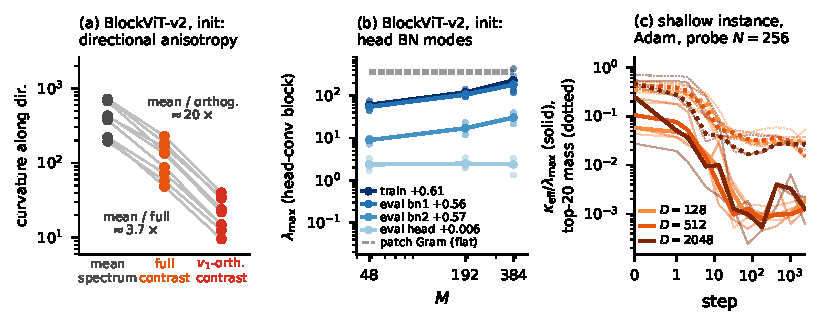
\includegraphics[width=\linewidth]{figures/fig2_diagnostics.pdf}}{\fbox{\rule{0pt}{2.2in}\rule{0.97\linewidth}{0pt}}}
\caption{Diagnostic limits. (a) BlockViT-v2 at initialization, no
optimizer: curvature along the mean-spectrum direction, the full
CancerEpi--CAS contrast and its $v_1$-orthogonal part (nine measurements).
(b) BlockViT-v2 at initialization: first-head-convolution block curvature
against width under four BatchNorm modes, with the flat incoming Gram
(dashed). (c) Shallow verified instance under Adam, probe $N=256$: the
residual's Rayleigh quotient relative to $\lambda_{\max}(K_\phip)$ (solid)
and its top-$20$ mass (dotted) along training.}
\label{fig:diagnostics}
\end{figure}
